
%=================================================================
%                           Start Document
%=================================================================
\sectiontitle{2}{Introduction}
\lhead{Introduction} % section header

\setstretch{1.6}


\subsection{Motivation}
\lhead{Introduction - Motivation}

Navigating biomedical instruments inside the brain remains challenging and high-risk due to the complexity and sensitivity of neural tissue. A range of neurological conditions, including epilepsy, parkinson's and brain tumors such as glioblastoma often necessitate interventions that require very high precision for localized drug delivery, thermal ablation, targeted stimulation or intracranial monitoring. Epilepsy alone affects around 50 million people globally \cite{noauthor_epilepsy_nodate}, and for nearly a third of them, medication alone is not enough to control seizures \cite{sultana_incidence_2021}. Glioblastoma, one of the most aggressive forms of brain cancer is diagnosed in approximately 150 000 people each year \cite{walsh_chapter_2016} where of many cases are deemed inoperable with traditional surgical tools. Finally many of the 10 million worldwide parkinsons patients \cite{noauthor_statistics_nodate} rely on precise deep brain stimulation to alleviate debilitating symptoms. There is thus a a clear real-world benefit to be made by improving the precision, safety, and accessibility of technologies that enable minimally invasive, targeted brain interventions.
\newline \newline
Robotic-assisted surgery has transformed many fields, but its application in neurosurgery remains limited by current technology \cite{doulgeris_robotics_2015}.The traditional rigid instruments are restricted in their ability to navigate delicate and structurally complex soft tissues such as the brain \cite{noseda_flat_2024}. Steerable, flexible devices offer a potential solution, improving access and safety while enabling new procedures \cite{da_veiga_challenges_2020}. Small-scale robotic devices, particularly those designed for transcranial access (see figure  offer a new way to reach deep seated brain regions with minimal disruption.

\begin{figure} [H]
    \centering
    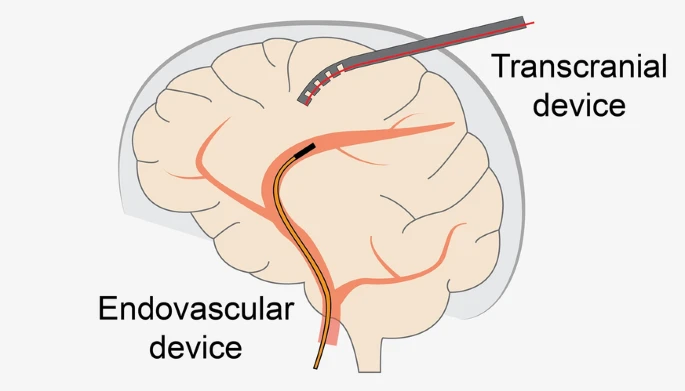
\includegraphics[width=0.8\linewidth]{images/brainsurgery/endovascularVsTranscranial.png}
    \caption{Caption}
    \label{fig:enter-label}
\end{figure}


Additionally, advancements in microfabrication have enabled the production of microscopic probes capable of monitoring biological activity and delivering stimulation or therapy \cite{chen_neural_2017} \cite{frank_next-generation_2019}. Yet, no steerable device has been developed that can both navigate brain tissue and utilize this technology for real-time sensin and targeted therapy. 
\newline \newline
To address this unmet need the MICROBS lab has developed a novel ribbon-shaped, tendon-driven continuum microrobot for minimally invasive neurosurgical interventions. This design allows for agile 3D navigation by achieving configuration unattainable by traditional rod-like instruments \cite{noseda_flat_2024}. Enabling precise navigation through soft tissue, capable of safely avoiding critical structures and reaching multiple target in a single insertion. However, this unique geometry introduces new challenges in modeling and control, requiring specialized solutions. Recognizing this need, the aim of this thesis is to develop closed-loop navigation for this novel robotic device enabling future effective use of this technology for brain surgery. 


%%\subsection{Background}
%%\lhead{Introduction - Background}



\lhead{Introduction - Project Interpretation}
\subsection{Project Interpretation}

This project aims to develop a closed-loop navigational system for a ribbon-shaped robotic device in brain tissue. In addition several preliminary tasks, outlined as  as steps 1-4 in the project description, needed to be completed before moving on to the closed loop design. The number of required tasks made the scope of the project quite broad. However, the primary goal from the outset was to produce reliable, well-documented work rooted in established theory. Early in the project, it was therefore agreed that if necessary, certain tasks could be scaled back or omitted to allow for a more thorough solution to the remaining ones. This was considered an important tradeoff to ensure that the project could serve as a solid foundation for further development and function as a robust proof of concept that could be used for demonstration to both clinicians and engineers.
\newline \newline
To the best of the author's knowledge, this is the first system of its kind and it thereby poses new and significant control challenges. As such, it was expected that a substantial portion of the project would need to be spent on developing the mathematical foundations of the system. Given the project's limited timeframe and the number of prerequisite tasks required before addressing the core navigation problem, it was decided that focus would be on implementing a robust 2D control strategy rather than rushing to implement a full 3D solution. Since the system will most likely be expanded upon or altered later on, special attention was  given to implementing the system in a robust and modular way in the codebase. Therefore the first step of refactoring was deemed essential. The overall goal being to deliver a reusable, scalable system that avoids the need for major rework in future development, rather than pursuing a more complex solution at the cost of quality or maintainability. 
\newline \newline
Although the focus is on robust implementation, the aim was also to explore how theoretically the system may be further developed and scaled in order to achieve optimal performance. Therefore this thesis also details the ways in which the modules may be expanded upon in further revisions and the mathematical concepts that may be employed later on. It also includes some ideas for the last point in the project description which is extension of the 2D control framework into 3D.

\subsection{Project Context}
\lhead{Introduction - Project Context}

This thesis builds upon an ongoing project at the MICROBS lab at EPFL towards developing a novel ribbon-shaped, tendon-driven continuum microrobot for minimally invasive neurosurgical interventions. The request for a closed loop control mechanism for the device came from Lorenzo Noseda who designed the device 

.....




\subsection{Contributions}
\lhead{Introduction - Contributions}

.....


\subsection{Outline}
\lhead{Introduction - Outline}
This work is structured into first the introduction which outlines the motivation behind the research, the project scope and objectives. Thereafter there is a Hardware section that describes the physical hardware that is used for the subsequent development.
\newline \newline 
The main body of the thesis is divided into five core topics corresponding to tasks 1-5 in the project description. These sections generally include methods, implementation and discussion with some also featuring design and further work subsections.
\newline \newline 
The first topic is software refactoring, detailing the methodology for the restructuring and development of the software framework. The second section describes how the tip tracking vision system was refactored and integrated with the control system. The third section focuses on how the existing path planning system was integrated with the 2D path following system. The fourth topic explains how the closed-loop tension control for the individual tendons was implemented and discusses its performance. The fifth and final section addresses the final 2D path following system, describing the design, kinematic modeling, implementation, and evaluation of the closed-loop system, along with an interpretation of the results, and discussion on possible further work.
\newline \newline
Conclusion wise, there is brief section which summarizes the project and reflects on the insights gained throughout the process.


%==============================================================
%                           End Document
%==============================================================
